\documentclass[aspectratio=169, 10pt]{beamer}

\usetheme{metropolis}
\usepackage{booktabs}
\usepackage{graphicx}
\usepackage{multirow}
\usepackage{array}
\usepackage{appendixnumberbeamer}
\usepackage{amsmath,amssymb}
\usepackage[backend=biber]{biblatex}
\addbibresource{references.bib}

% ── Colour palette ──────────────────────────────────
\definecolor{PrimaryBlue}{HTML}{1A73E8}
\definecolor{AccentTeal}{HTML}{00897B}
\definecolor{DarkBg}{HTML}{23272F}
\definecolor{LightGray}{HTML}{F5F5F5}

\setbeamercolor{palette primary}{bg=PrimaryBlue}
\setbeamercolor{frametitle}{bg=PrimaryBlue, fg=white}
\setbeamercolor{title separator}{fg=AccentTeal}
\setbeamercolor{progress bar}{fg=AccentTeal, bg=LightGray}
\setbeamercolor{block title}{bg=AccentTeal, fg=white}
\setbeamercolor{alerted text}{fg=AccentTeal}

\setbeamerfont{title}{series=\bfseries, size=\Large}
\setbeamerfont{frametitle}{series=\bfseries}

% ── Meta ────────────────────────────────────────────
\title{Exploring Human Steering Performance\\on Complex 3D Paths}
\subtitle{A Requirements Analysis for a Human-Centered Evaluation System}
\author{
  Yousuf Ibne Kamal Niloy \and
  Samnun Azfar \and
  Anika Farzana \and
  Yousef Fuad Ahmed Al-Khasheb
}
\institute{
  Department of Computer Science and Engineering\\
  Islamic University of Technology (IUT), OIC
}
\date{CSE 6275 / CSE 6391: AHCI --- Assignment 1}

% ═══════════════════════════════════════════════════
\begin{document}

% ── 1  Title ────────────────────────────────────────
\begin{frame}[plain]
  \titlepage
\end{frame}

% ── 2  Outline ──────────────────────────────────────
\begin{frame}{Outline}
  \tableofcontents
\end{frame}

% ━━━━━━━━━━━━━━━━━━━━━━━━━━━━━━━━━━━━━━━━━━━━━━━━━
\section{Introduction}
% ━━━━━━━━━━━━━━━━━━━━━━━━━━━━━━━━━━━━━━━━━━━━━━━━━

% ── 3  Background ───────────────────────────────────
\begin{frame}{Background \& Motivation}
  \begin{itemize}
    \item \textbf{Steering Law} extends Fitts' Law to trajectory-based tasks:\\
          $MT = a + b \cdot \dfrac{L}{W}$
    \item Modern systems increasingly involve \alert{complex 3D environments}:\\
          VR, simulation training, 3D design, robotic teleoperation
    \item Existing models focus on 2D or simple straight 3D paths
    \item Path \emph{curvature} and \emph{complexity} significantly affect performance
    \item \textbf{Human-Centered Machine Learning (HCML)} aims to model and support
          human behaviour while preserving transparency and user control
  \end{itemize}
\end{frame}

% ── 4  Objectives ───────────────────────────────────
\begin{frame}{Objectives \& Contributions}
  \textbf{Objectives}
  \begin{enumerate}
    \item Port Chen et.\ al's emperical approach of emperical evaluation of a modified fitts law to 3D curves \cite{chen2025curves}
    \item Identify use cases for a 3D steering evaluation system
    \item Develop personas to validate and ground the identified use cases
  \end{enumerate}

  \vspace{0.5em}
  \textbf{Key Contributions}
  \begin{itemize}
    \item Empirical understanding of 3D steering challenges
    \item Personas demonstrating meaningful use of the 3D adaptation
  \end{itemize}
\end{frame}


% ━━━━━━━━━━━━━━━━━━━━━━━━━━━━━━━━━━━━━━━━━━━━━━━━━
\section{Related Work}
% ━━━━━━━━━━━━━━━━━━━━━━━━━━━━━━━━━━━━━━━━━━━━━━━━━

% ── 5  Related Work ─────────────────────────────────
\begin{frame}{Related Work \& Theoretical Background}
  \begin{columns}[T]
    \begin{column}{0.48\textwidth}
      \textbf{HCI Foundations}
      \begin{itemize}
        \item Interaction design: personas, scenarios, task analysis
        \item Goal-directed design for usable systems
      \end{itemize}

      \vspace{0.6em}
      \textbf{Steering Law}
      \begin{itemize}
        \item Accot \& Zhai (1997): trajectory-based movement model
        \item Extensions for curvature, path complexity
        \item Limited 3D validation
      \end{itemize}
    \end{column}
    \begin{column}{0.48\textwidth}
      \textbf{HCML \& Trajectory Prediction}
      \begin{itemize}
        \item Deep learning for human trajectory prediction
        \item ML for VR and teleoperation behaviour modelling
        \item Focus on transparency, interpretability \& human oversight
      \end{itemize}
    \end{column}
  \end{columns}
\end{frame}

% ━━━━━━━━━━━━━━━━━━━━━━━━━━━━━━━━━━━━━━━━━━━━━━━━━
\section{Methodology}
% ━━━━━━━━━━━━━━━━━━━━━━━━━━━━━━━━━━━━━━━━━━━━━━━━━

% ── 6  Data Gathering ───────────────────────────────
\begin{frame}{Methodology: Data Gathering}
  \begin{columns}[T]
    \begin{column}{0.48\textwidth}
      \textbf{Data Gathering Methods}
      \begin{itemize}
        \item Systematic literature review
        \item Secondary source analysis
        \item AI-supported knowledge synthesis
        \item Researcher reflexive analysis
      \end{itemize}
    \end{column}
    \begin{column}{0.48\textwidth}
      \textbf{Ethical Considerations}
      \begin{itemize}
        \item Informed consent
        \item Anonymity \& privacy
        \item Secure data protection
        \item Participant well-being
        \item AI-specific ethical safeguards
      \end{itemize}
    \end{column}
  \end{columns}
\end{frame}

% ── 7  Stakeholders ─────────────────────────────────
\begin{frame}{Stakeholder Identification}
  \begin{description}
    \item[\color{PrimaryBlue}Primary]~\\
      HCI Researchers \(\cdot\) Study Participants \(\cdot\) System Operators
    \item[\color{AccentTeal}Secondary]~\\
      VR / 3D Interface Designers \(\cdot\) Academic Researchers
    \item[Indirect]~\\
      End-users of future 3D systems (VR, simulation, training)
  \end{description}
\end{frame}

\begin{frame}{Porting from 2D to 3D}
  \begin{block}{The Formula for porting into 3D}
    \begin{align*}
        &x^2 + y^2 = r^2 \\
        &z = \sum_{i=1}^n \sin(a_ix+b_iy)
    \end{align*}
  \end{block}
\end{frame}

\begin{frame}{Comparison of 2D and #d approaches}
    \begin{figure}
        \centering
        \begin{minipage}{0.48\textwidth}
            \centering
            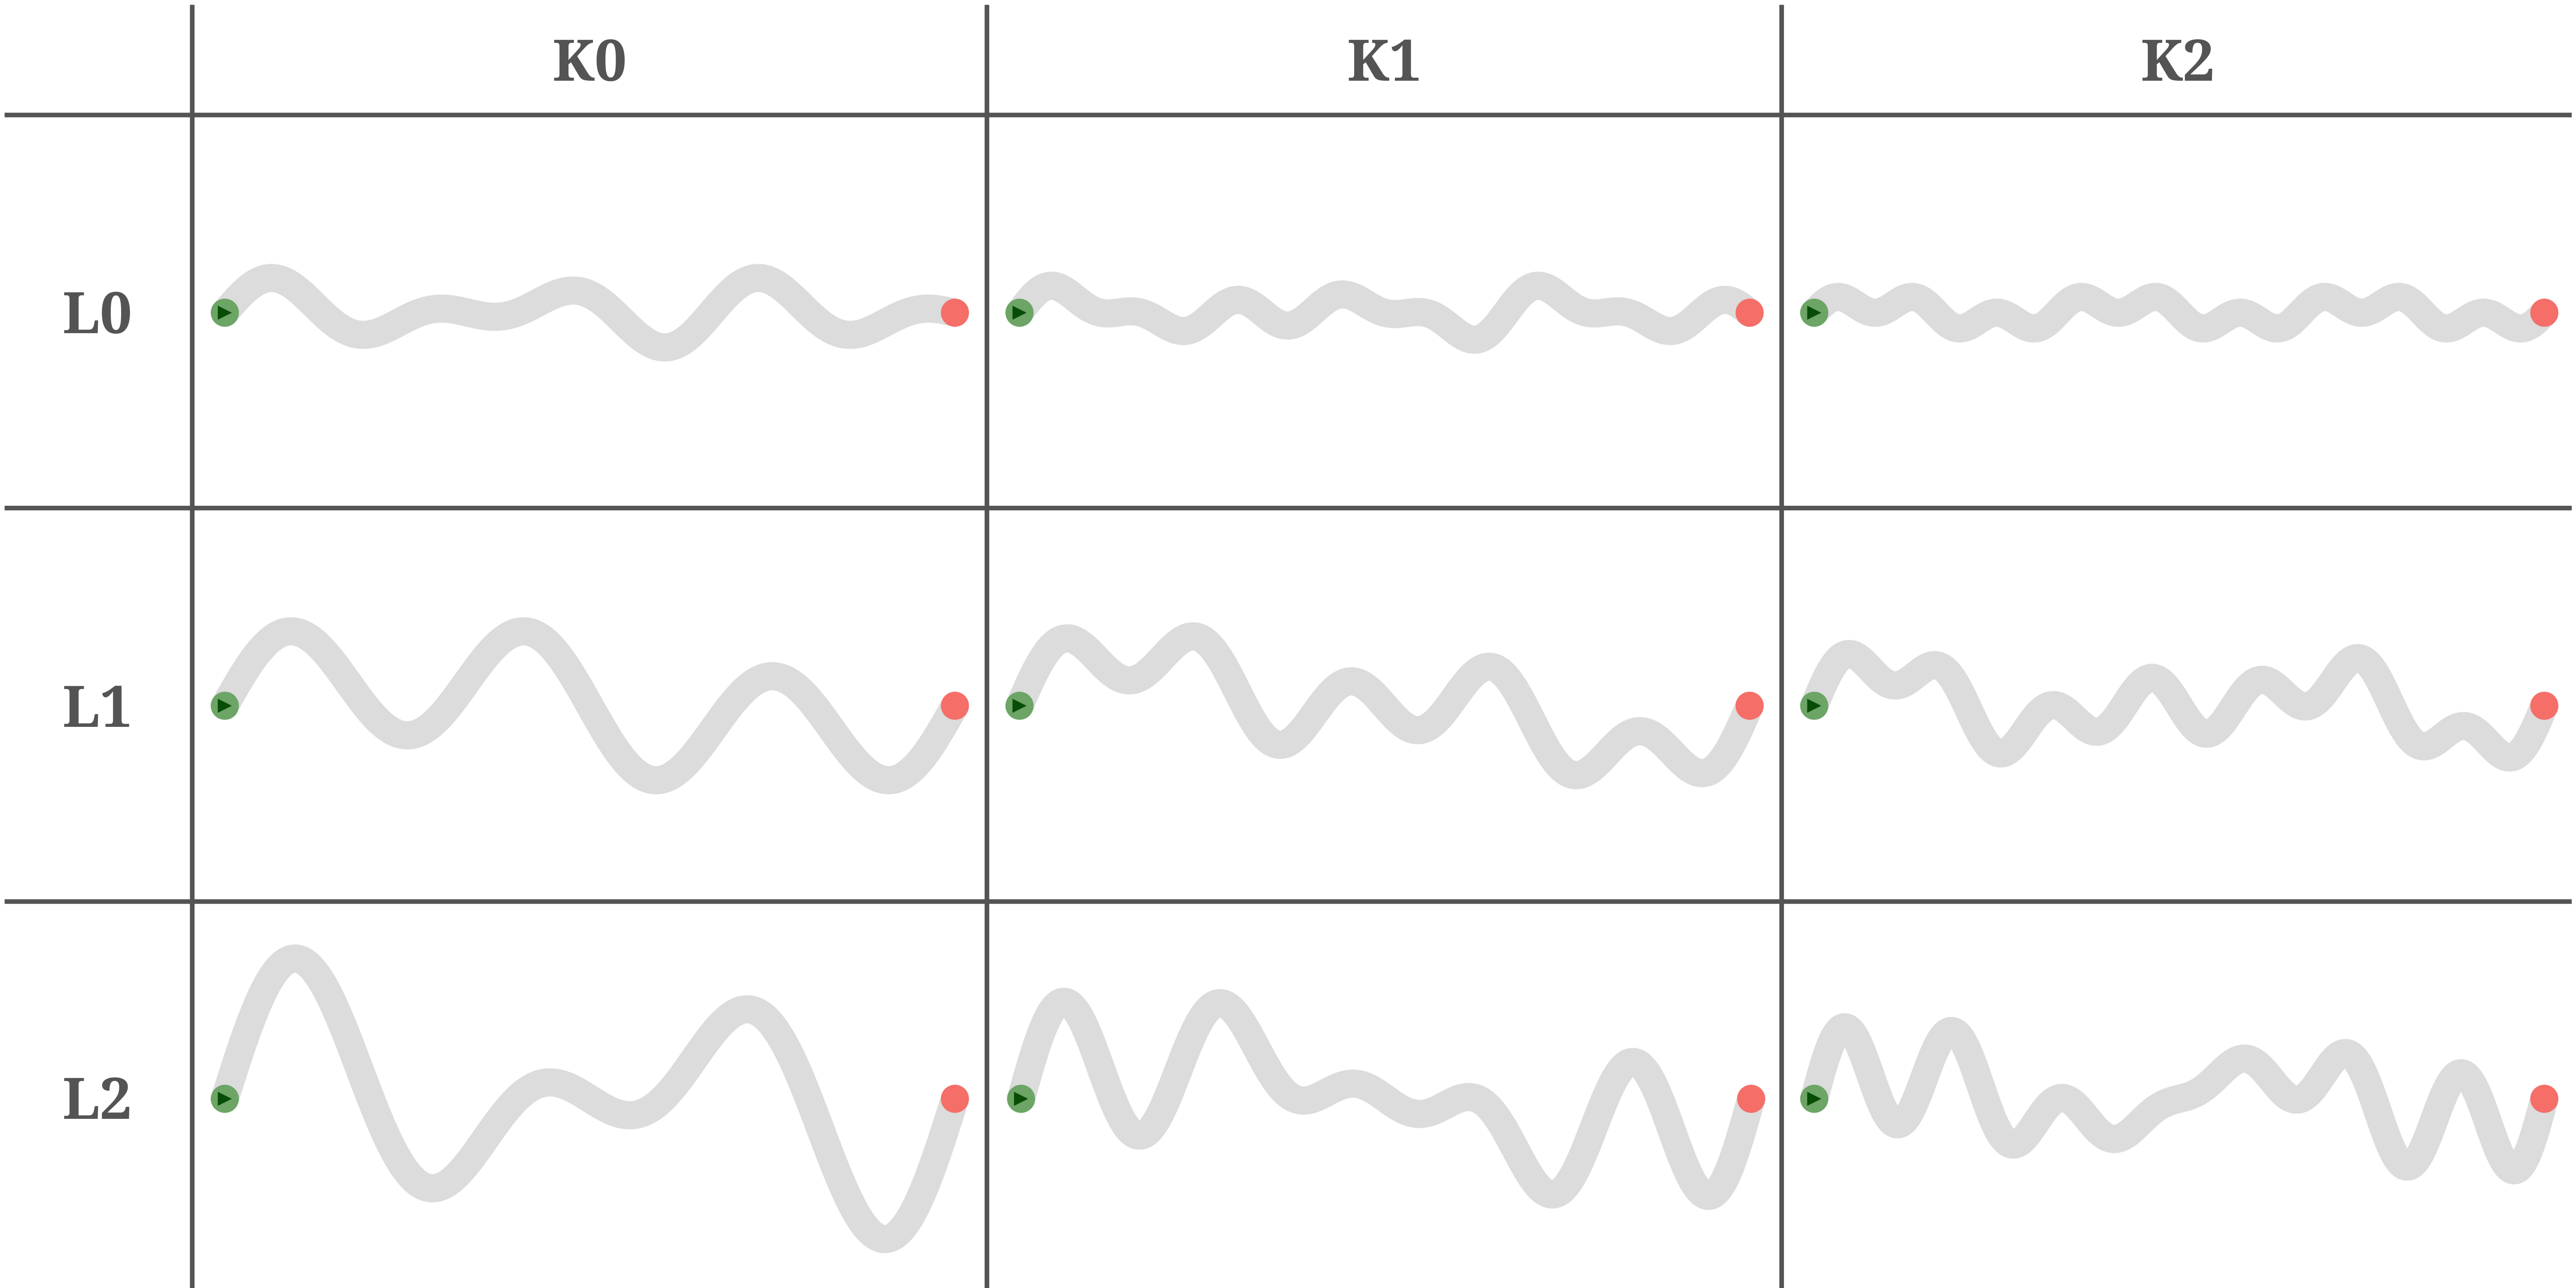
\includegraphics[width=\linewidth]{images/path_diagram.png}
            \caption{2D Path Diagram (as shown by Chen et.al.)}
        \end{minipage}\hfill
        \begin{minipage}{0.48\textwidth}
            \centering
            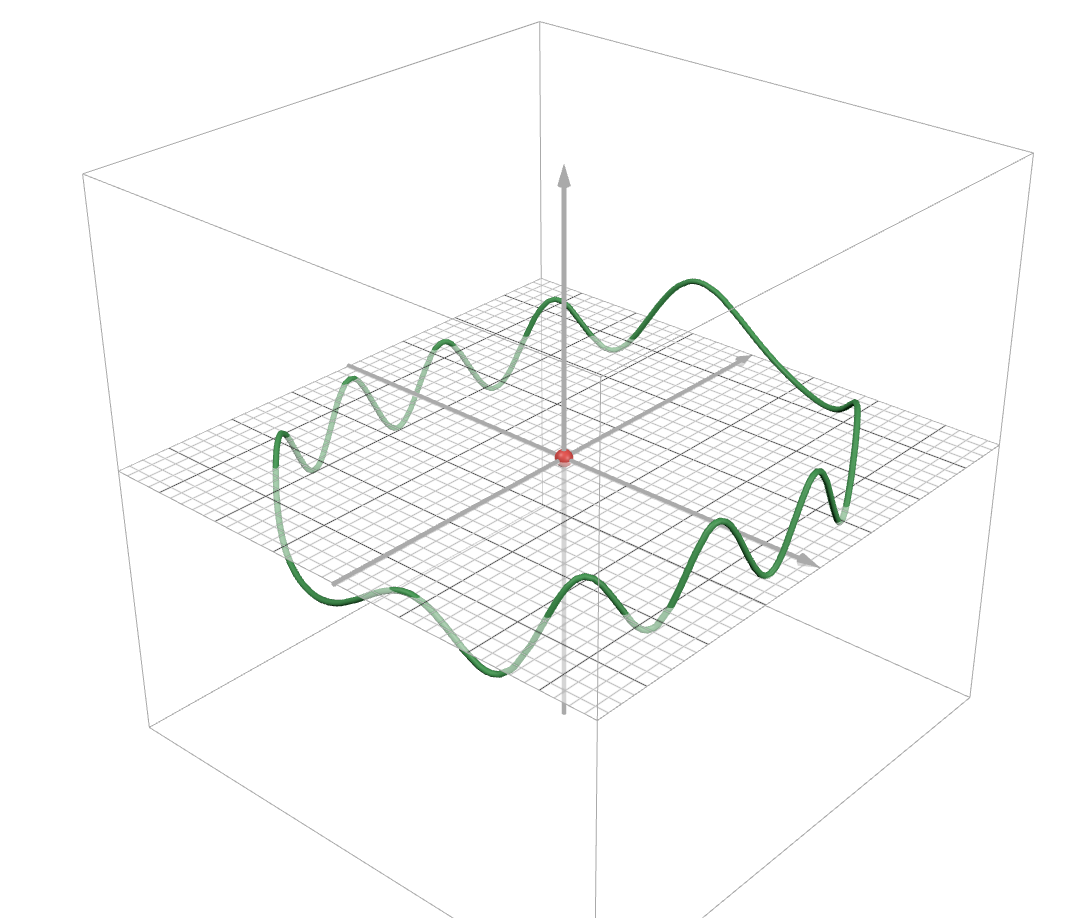
\includegraphics[width=\linewidth]{images/3d-conversion-of-trial.png}
            \caption{3D Conversion of the 2D path Diagram}
        \end{minipage}
    \end{figure}
\end{frame}



% ━━━━━━━━━━━━━━━━━━━━━━━━━━━━━━━━━━━━━━━━━━━━━━━━━
\section{Key Findings}
% ━━━━━━━━━━━━━━━━━━━━━━━━━━━━━━━━━━━━━━━━━━━━━━━━━

% ── 8  Key Findings ─────────────────────────────────
\begin{frame}{Key Findings}
  \begin{columns}[T]
    \begin{column}{0.48\textwidth}
      \textbf{User Goals \& Motivations}
      \begin{itemize}
        \item Reliable, reproducible performance measures
        \item Clear task structure \& meaningful feedback
        \item Intuitive interaction, low cognitive overhead
      \end{itemize}
      \vspace{0.5em}
      \textbf{Pain Points}
      \begin{itemize}
        \item No standardised 3D path representations
        \item Hard to compare across input devices
        \item Limited 3D trajectory visualisation
      \end{itemize}
    \end{column}
    \begin{column}{0.48\textwidth}
      \textbf{AI Attitudes}
      \begin{itemize}
        \item Valuable for pattern discovery
        \item Concerns about opaque automation
        \item Transparency \& explainability critical
      \end{itemize}
      \vspace{0.5em}
      \textbf{Contextual Constraints}
      \begin{itemize}
        \item Lab vs.\ non-lab contexts
        \item Hardware heterogeneity
        \item Recruitment \& scheduling
      \end{itemize}
    \end{column}
  \end{columns}
\end{frame}

% ━━━━━━━━━━━━━━━━━━━━━━━━━━━━━━━━━━━━━━━━━━━━━━━━━
\section{Personas}
% ━━━━━━━━━━━━━━━━━━━━━━━━━━━━━━━━━━━━━━━━━━━━━━━━━

% ── 9  Persona 1 ────────────────────────────────────
\begin{frame}{Persona 1: Experimental HCI Researcher (Primary)}
  \begin{columns}[T]
    \begin{column}{0.35\textwidth}
      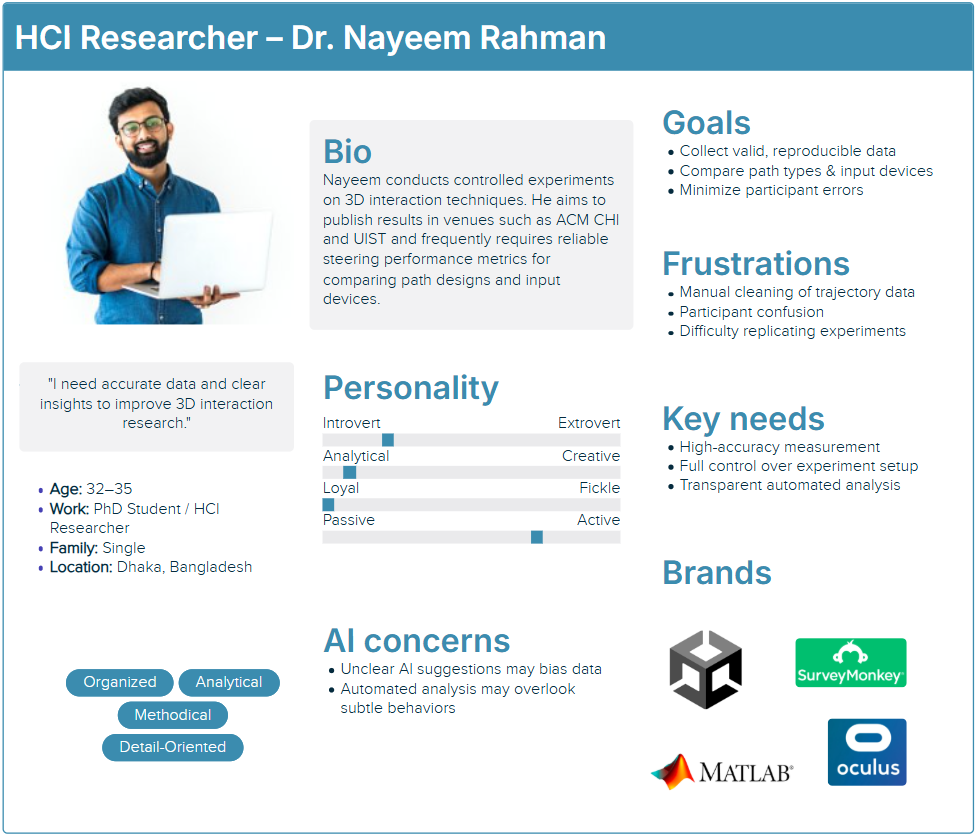
\includegraphics[width=\linewidth]{../report/images/Researcher.png}
    \end{column}
    \begin{column}{0.60\textwidth}
      \textbf{Dr.\ Nayeem Rahman}, 29, PhD Candidate\\[0.3em]
      \textbf{Skill:} High (Unity, statistics, experimental design)\\
      \textbf{Context:} University lab experiments\\[0.5em]
      \textbf{Goals:} Reliable \& reproducible data; compare path types\\[0.3em]
      \textbf{Pain Points:} Participant confusion; manual log cleaning; difficult reproducibility\\[0.3em]
      \textbf{AI Expectations:} Automated outlier detection; transparent analysis
    \end{column}
  \end{columns}
\end{frame}

% ── 10  Persona 2 ───────────────────────────────────
\begin{frame}{Persona 2: Lab Study Administrator (Support)}
  \begin{columns}[T]
    \begin{column}{0.35\textwidth}
      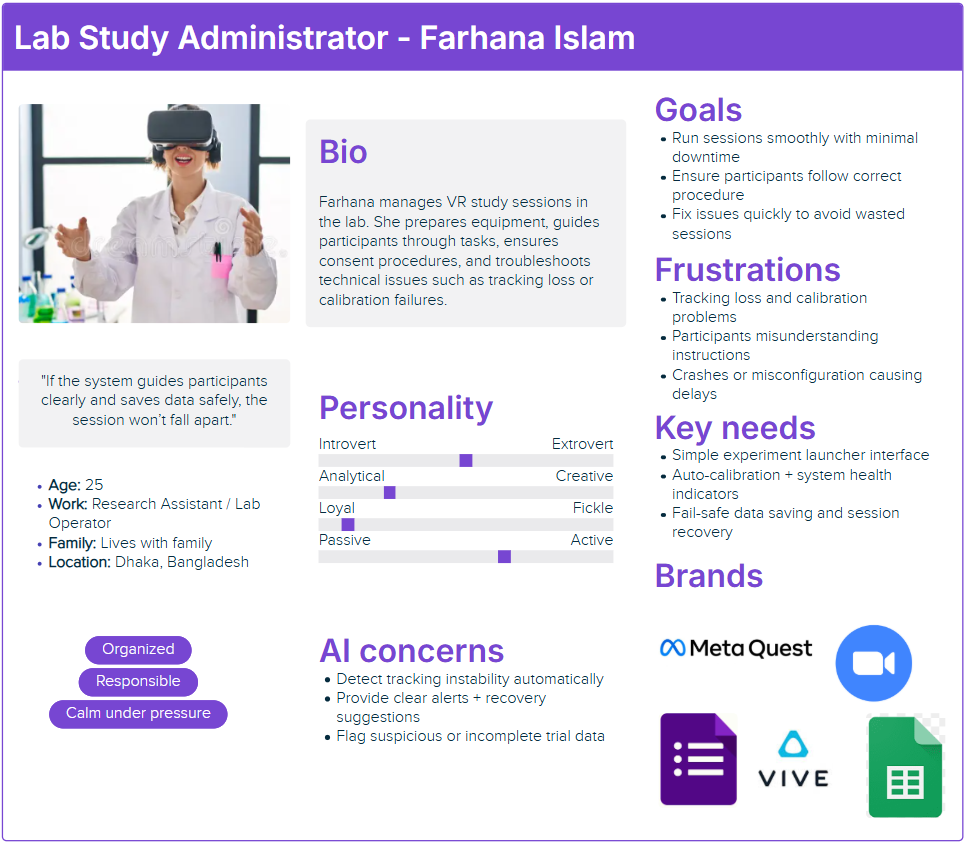
\includegraphics[width=\linewidth]{../report/images/LabOperator.png}
    \end{column}
    \begin{column}{0.60\textwidth}
      \textbf{Farhana Islam}, 25, Research Assistant\\[0.3em]
      \textbf{Skill:} Medium (VR setup, not advanced programming)\\
      \textbf{Context:} Physical lab, managing participants \& hardware\\[0.5em]
      \textbf{Goals:} Smooth sessions; correct procedures; quick issue resolution\\[0.3em]
      \textbf{Pain Points:} Tracking loss; participant confusion; crashes\\[0.3em]
      \textbf{AI Expectations:} Automatic instability detection; clear recovery alerts
    \end{column}
  \end{columns}
\end{frame}

% ── 11  Persona 3 ───────────────────────────────────
\begin{frame}{Persona 3: Skilled Gamer Participant (Secondary)}
  \begin{columns}[T]
    \begin{column}{0.35\textwidth}
      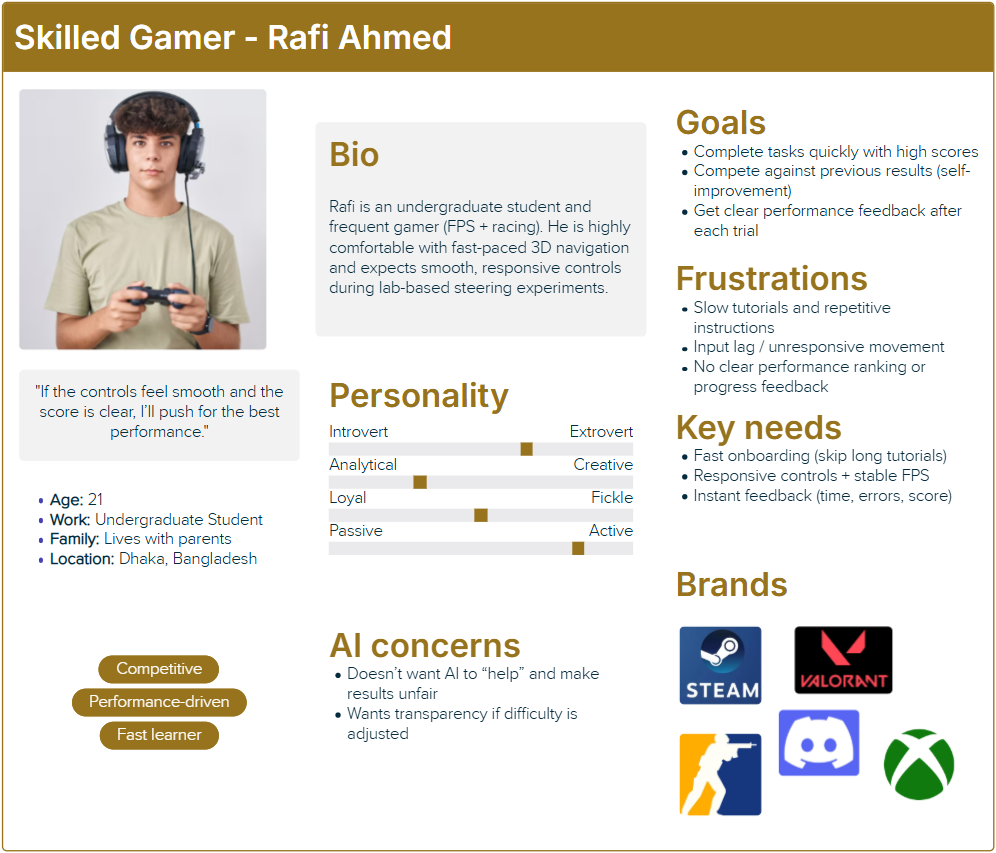
\includegraphics[width=\linewidth]{../report/images/Gamer.png}
    \end{column}
    \begin{column}{0.60\textwidth}
      \textbf{Rafi Ahmed}, 21, Undergraduate (frequent gamer)\\[0.3em]
      \textbf{Skill:} Medium-High\\
      \textbf{Context:} Lab study with competitive mindset\\[0.5em]
      \textbf{Goals:} Perform well; clear scoring; feel challenged\\[0.3em]
      \textbf{Pain Points:} Long tutorials; input lag; no performance comparison\\[0.3em]
      \textbf{AI Concerns:} Unfair difficulty adjustment
    \end{column}
  \end{columns}
\end{frame}

% ── 12  Persona 4 ───────────────────────────────────
\begin{frame}{Persona 4: VR Novice Participant (Secondary)}
  \begin{columns}[T]
    \begin{column}{0.35\textwidth}
      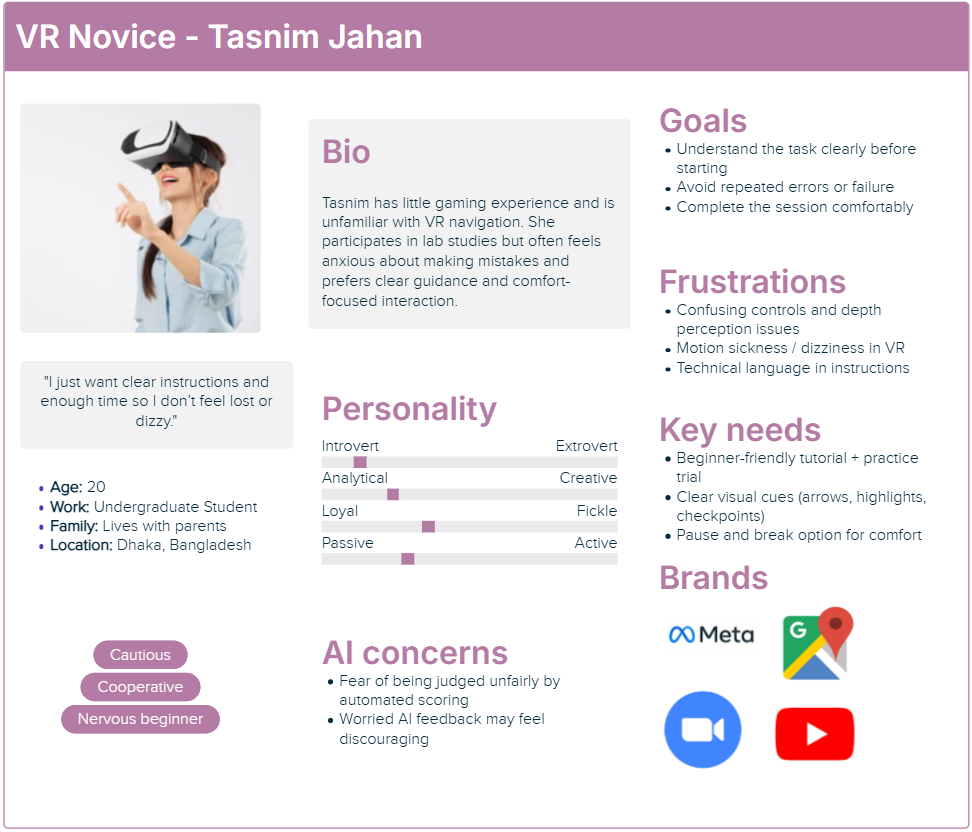
\includegraphics[width=\linewidth]{../report/images/VRNovice.png}
    \end{column}
    \begin{column}{0.60\textwidth}
      \textbf{Tasnim Jahan}, 20, Undergraduate (non-gamer)\\[0.3em]
      \textbf{Skill:} Low-Medium\\
      \textbf{Context:} Lab study, unfamiliar with VR\\[0.5em]
      \textbf{Goals:} Clear instructions; avoid failure; comfortable session\\[0.3em]
      \textbf{Pain Points:} Confusing controls; motion sickness; technical jargon\\[0.3em]
      \textbf{AI Concerns:} Fear of being judged by AI scoring
    \end{column}
  \end{columns}
\end{frame}

% ── 13  Persona 5 ───────────────────────────────────
\begin{frame}{Persona 5: Accessibility-Constrained (Edge)}
  \begin{columns}[T]
    \begin{column}{0.35\textwidth}
      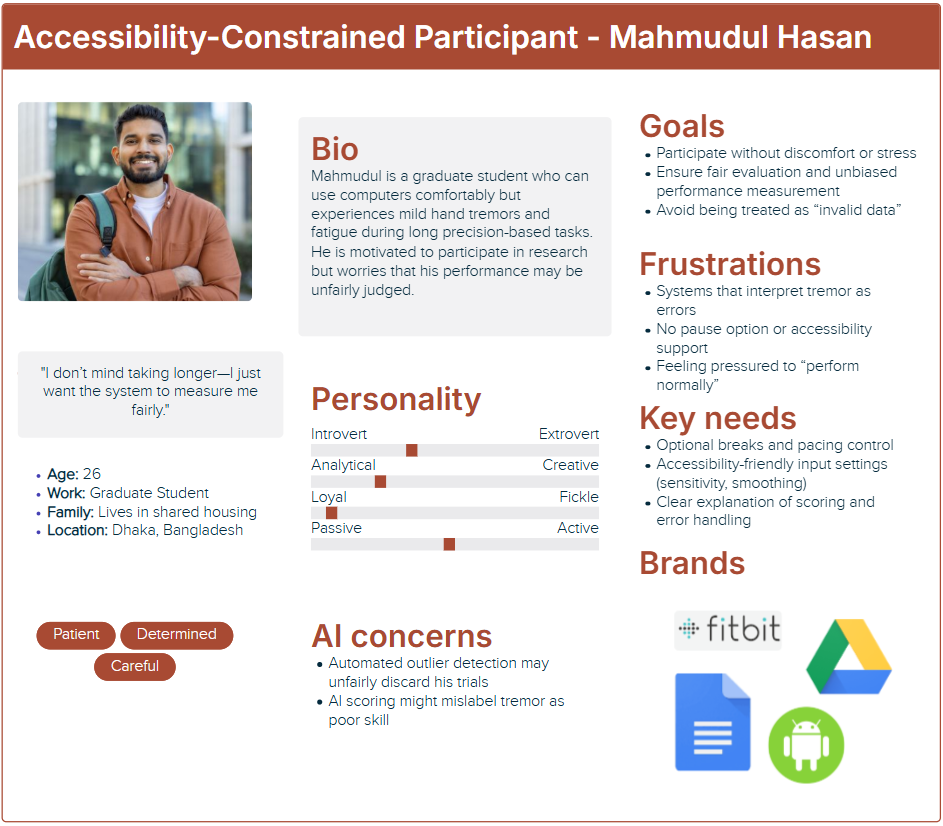
\includegraphics[width=\linewidth]{../report/images/AccessibilityParticipant.png}
    \end{column}
    \begin{column}{0.60\textwidth}
      \textbf{Mahmudul Hasan}, 26, Graduate Student\\[0.3em]
      \textbf{Skill:} Medium \quad \textbf{Constraint:} Mild hand tremor\\
      \textbf{Context:} Lab study with fatigue sensitivity\\[0.5em]
      \textbf{Goals:} Participate without discomfort; fair evaluation\\[0.3em]
      \textbf{Pain Points:} Tremor interpreted as errors; no pause/accessibility support\\[0.3em]
      \textbf{AI Concerns:} Outlier detection may unfairly discard trials
    \end{column}
  \end{columns}
\end{frame}

% ━━━━━━━━━━━━━━━━━━━━━━━━━━━━━━━━━━━━━━━━━━━━━━━━━
\section{Scenarios \& Task Analysis}
% ━━━━━━━━━━━━━━━━━━━━━━━━━━━━━━━━━━━━━━━━━━━━━━━━━

% ── 14  Scenarios ───────────────────────────────────
\begin{frame}{Usage Scenarios}
  \small
  \begin{tabular}{@{}l l p{6.5cm}@{}}
    \toprule
    \textbf{\#} & \textbf{Persona} & \textbf{Scenario Highlights} \\
    \midrule
    1 & Dr.\ Nayeem & Configure experiment, pilot study, HCML-assisted curvature--error analysis \\
    2 & Farhana    & Checklist launch, tracking-loss auto-pause, session report \\
    3 & Rafi       & Quick onboarding, speed--accuracy trade-off, real-time feedback \\
    4 & Tasnim     & Guided tutorial, break support, simple performance explanation \\
    5 & Mahmudul   & Accessibility mode, widened tolerance, transparent outlier review \\
    \bottomrule
  \end{tabular}

  \vspace{0.8em}
  Each scenario illustrates \textbf{normal use}, \textbf{ML-assisted insight}, \textbf{accessibility}, or \textbf{operational workflows} --- ensuring ML supports, not replaces, human decision-making.
\end{frame}

% ── 15  Task Analysis ───────────────────────────────
\begin{frame}{Hierarchical Task Analysis}
  \textbf{Primary Task:} \emph{Complete a 3D Steering Trial}

  \begin{columns}[T]
    \begin{column}{0.48\textwidth}
      \begin{enumerate}
        \item \textbf{Receive Instructions}\\
              Read description, learn controls
        \item \textbf{Complete Practice Trial}\\
              Navigate practice path, get feedback
        \item \textbf{Execute Experimental Trial}\\
              Position → steer → reach end point
        \item \textbf{Receive Feedback}\\
              Metrics, comparison, prepare next
      \end{enumerate}
    \end{column}
    \begin{column}{0.48\textwidth}
      \textbf{HCML Support Opportunities}
      \begin{itemize}
        \item ML modelling of movement time \& deviation
        \item Detection of low-quality trials
        \item Steering strategy clustering
        \item Interpretable visual summaries
      \end{itemize}
      \vspace{0.5em}
      \textbf{Risks}
      \begin{itemize}
        \item Model bias with small datasets
        \item Correlation ≠ causation
        \item Over-reliance on automation
      \end{itemize}
    \end{column}
  \end{columns}
\end{frame}

% ━━━━━━━━━━━━━━━━━━━━━━━━━━━━━━━━━━━━━━━━━━━━━━━━━
\section{Requirements}
% ━━━━━━━━━━━━━━━━━━━━━━━━━━━━━━━━━━━━━━━━━━━━━━━━━

% ── 16  Functional Requirements ─────────────────────
\begin{frame}{Functional Requirements (FR1--FR12)}
  \small
  \begin{columns}[T]
    \begin{column}{0.48\textwidth}
      \begin{description}
        \item[FR1] Built in Unity engine
        \item[FR2] Configurable 3D path geometry
        \item[FR3] Mouse \& VR controller input
        \item[FR4] Millisecond-precision timing
        \item[FR5] Boundary violation detection
        \item[FR6] High-rate trajectory capture
      \end{description}
    \end{column}
    \begin{column}{0.48\textwidth}
      \begin{description}
        \item[FR7] Tutorial \& practice trials
        \item[FR8] Automatic trial randomisation
        \item[FR9] CSV / JSON data export
        \item[FR10] Descriptive stats \& ML-ready data
        \item[FR11] Meta VR headset support
        \item[FR12] Standard mouse input support
      \end{description}
    \end{column}
  \end{columns}
\end{frame}

% ── 17  Non-Functional Requirements ─────────────────
\begin{frame}{Non-Functional \& Other Requirements}
  \begin{columns}[T]
    \begin{column}{0.48\textwidth}
      \textbf{Non-Functional (NFR1--NFR8)}
      \begin{itemize}
        \item ≥ 60 FPS on GTX 1650
        \item Sub-perceptual input latency
        \item Windows 10+; Meta VR headsets
        \item Tutorial ≤ 3 min; data loss < 0.1\%
        \item Full logging for reproducibility
        \item Secure \& anonymised storage
      \end{itemize}
    \end{column}
    \begin{column}{0.48\textwidth}
      \textbf{User (UR1--UR4)}
      \begin{itemize}
        \item Visual path following on screen/VR
        \item Mouse or VR controller capable
        \item Researcher: experimental design knowledge
        \item Operator: basic Unity familiarity
      \end{itemize}
      \vspace{0.4em}
      \textbf{Data \& Environmental (DER1--DER4)}
      \begin{itemize}
        \item ≥ 60 Hz sampling; Quest headsets
        \item Min spec: i5, 8 GB, GTX 1650
        \item 100 MB storage per participant
      \end{itemize}
    \end{column}
  \end{columns}
\end{frame}

% ━━━━━━━━━━━━━━━━━━━━━━━━━━━━━━━━━━━━━━━━━━━━━━━━━
\section{Usability \& UX Goals}
% ━━━━━━━━━━━━━━━━━━━━━━━━━━━━━━━━━━━━━━━━━━━━━━━━━

% ── 18  Usability & UX ──────────────────────────────
\begin{frame}{Usability \& User Experience Goals}
  \begin{columns}[T]
    \begin{column}{0.48\textwidth}
      \textbf{Usability Goals}
      \begin{itemize}
        \item \textbf{Effectiveness:} ≥ 95\% trial completion without help
        \item \textbf{Efficiency:} Setup < 5 min; experiment config < 10 min
        \item \textbf{Learnability:} Stable performance within 3 practice trials
        \item \textbf{Error Tolerance:} Auto-recovery; zero data loss from SW failure
        \item \textbf{Data Integrity:} Synchronised timestamps; verified logs
      \end{itemize}
    \end{column}
    \begin{column}{0.48\textwidth}
      \textbf{Experiential Goals}
      \begin{itemize}
        \item \textbf{Trust:} ≥ 85\% agreement on fair measurement
        \item \textbf{Confidence:} Transparent logs \& visualisations
        \item \textbf{Control:} Latency < 50 ms; ≥ 60 FPS
        \item \textbf{ML Transparency:} Explainable automated analysis
        \item \textbf{Engagement:} Breaks, progress indicators
        \item \textbf{Ethics:} Full informed consent; no PII stored
      \end{itemize}
    \end{column}
  \end{columns}
\end{frame}

% ━━━━━━━━━━━━━━━━━━━━━━━━━━━━━━━━━━━━━━━━━━━━━━━━━
\section{Traceability \& Volere Shells}
% ━━━━━━━━━━━━━━━━━━━━━━━━━━━━━━━━━━━━━━━━━━━━━━━━━

% ── 19  Traceability Matrix ─────────────────────────
\begin{frame}{Requirements--Goals Traceability Matrix}
  \scriptsize
  \begin{tabular}{@{}p{2.8cm} p{3.5cm} p{2.8cm} p{2.8cm}@{}}
    \toprule
    \textbf{User Goal} & \textbf{Persona / Scenario} & \textbf{Req.\ ID} & \textbf{UX Goal} \\
    \midrule
    Collect reliable data        & P1 -- Researcher (S1) & FR4,5,6; NFR6 & Effectiveness, Trust \\
    Configure experiments        & P1 -- Researcher (S1) & FR1,2,8; UR3  & Efficiency, Learnability \\
    Run sessions smoothly        & P2 -- Operator (S2)   & FR7,9; NFR7; DER2 & Efficiency, Confidence \\
    Prevent data loss            & P2 -- Operator (S2)   & NFR7,8; FR9   & Trust, Reliability \\
    Understand tasks clearly     & P4 -- Novice (S4)     & FR7; UR1; NFR5 & Learnability, Comfort \\
    Complete trials quickly      & P3 -- Gamer (S3)      & NFR1,2; FR3   & Efficiency, Engagement \\
    Participate w/o discomfort   & P5 -- Access.\ (S5)   & UR1; DER1; NFR5 & Comfort, Control \\
    Ensure fair evaluation       & P5 -- Access.\ (S5)   & NFR6; FR10    & Trust, Transparency \\
    \bottomrule
  \end{tabular}
\end{frame}

% ── 20  Volere Shells ───────────────────────────────
\begin{frame}{Volere Requirement Shells (Examples)}
  \begin{columns}[T]
    \begin{column}{0.48\textwidth}
      \textbf{FR5 -- Boundary Violation Detection}
      \begin{itemize}
        \item \textbf{Type:} Functional
        \item \textbf{Description:} Detect \& count boundary violations during steering
        \item \textbf{Rationale:} Key performance metric for steering law experiments
        \item \textbf{Fit Criterion:} ≥ 99\% detection accuracy
        \item \textbf{Priority:} High
        \item \textbf{Dependencies:} FR2, DER1
      \end{itemize}
    \end{column}
    \begin{column}{0.48\textwidth}
      \textbf{NFR1 -- Performance (FPS)}
      \begin{itemize}
        \item \textbf{Type:} Non-Functional
        \item \textbf{Description:} Maintain ≥ 60 FPS on GTX 1650
        \item \textbf{Rationale:} Stable FPS ensures accurate measurement \& avoids latency bias
        \item \textbf{Fit Criterion:} FPS ≥ 60 in 95\% of trials
        \item \textbf{Priority:} High
        \item \textbf{Dependencies:} FR2, FR3
      \end{itemize}
    \end{column}
  \end{columns}
\end{frame}

% ━━━━━━━━━━━━━━━━━━━━━━━━━━━━━━━━━━━━━━━━━━━━━━━━━
\section{Discussion \& Conclusion}
% ━━━━━━━━━━━━━━━━━━━━━━━━━━━━━━━━━━━━━━━━━━━━━━━━━

% ── 21  Design Trade-offs ───────────────────────────
\begin{frame}{Design Trade-offs \& Implications}
  \begin{itemize}
    \item \textbf{Model Adaptivity vs.\ Experimental Control}\\
          Adaptive ML may introduce bias --- must be optional \& fully logged
    \item \textbf{Data Richness vs.\ System Performance}\\
          High-frequency logging improves ML but increases compute load
    \item \textbf{Automation vs.\ Human Oversight}\\
          Researchers must remain in control of model selection \& interpretation
    \item \textbf{Standardisation vs.\ Model Generalisation}\\
          Standard paths aid reproducibility; diverse paths aid ML generalisation
  \end{itemize}

  \vspace{0.5em}
  \alert{System will NOT support:} Fully autonomous design; real-time protocol changes; black-box models without interpretability.
\end{frame}

% ── 22  Limitations & Future Work ───────────────────
\begin{frame}{Limitations \& Future Work}
  \begin{columns}[T]
    \begin{column}{0.48\textwidth}
      \textbf{Limitations}
      \begin{itemize}
        \item Personas from literature, not large-scale empirical data
        \item ML requirements may evolve post-prototype
        \item Hardware scope limited to mid-range \& Meta VR
        \item Limited cross-cultural analysis
      \end{itemize}
    \end{column}
    \begin{column}{0.48\textwidth}
      \textbf{Future Work}
      \begin{itemize}
        \item Unity-based prototype for data collection
        \item ML models for movement time \& error prediction
        \item Interpretable steering behaviour models
        \item Pilot user studies to validate requirements
        \item Adaptive feedback guided by HCML principles
      \end{itemize}
    \end{column}
  \end{columns}
\end{frame}

% ── 23  Conclusion ──────────────────────────────────
\begin{frame}{Conclusion}
  \begin{itemize}
    \item Presented a \textbf{structured requirements analysis} for an HCML system
          to study human steering in complex 3D environments
    \item Developed \textbf{5 personas} and \textbf{5 aligned scenarios} grounded in
          human-centred design
    \item Specified \textbf{functional, non-functional, user, data \& environmental}
          requirements with traceability
    \item Emphasised \textbf{transparency, interpretability, human oversight} and
          \textbf{ethical data handling}
    \item Provides a foundation for \textbf{predictive modelling} of 3D steering
          performance and \textbf{adaptive, human-centred systems}
  \end{itemize}

  \vspace{1em}
  \centering
  {\Large\bfseries Thank You!}\\[0.3em]
  Questions?
\end{frame}

% ── References ──────────────────────────────────────
\begin{frame}[allowframebreak]{References}
  \printbibliography[heading=none]
\end{frame}

\end{document}
